\chapter{Basics of response modeling}

\section{Amorphous track models}
ATMs (in a slightly confusing manner also referred to as 'track structure
models') started from the works of Robert Katz in the late 1950s. He and his
team worked on finding magnetic monopoles in nuclear emulsions exposed to
high-altitute cosmic radiation (TODO Ref.). Soon, \ldots

ATMs rely on two major assumptions:

\begin{list}
\item{}They disregard the stochastic energy deposition pattern by secondary
electrons around the track of heavy charged particles (protons or
ions, HCPs). Instead, the averaged dose $d$ as a function of
distance $r$ from the trajectory is considered. $d(r)$ is mostly referred as the
'radial dose distribution' although the term 'distribution' is not fully correct
(Fig. \ref{fig:TST}).
\item{}The second important assumption is that -- since photons deposit their
energy eventually by electrons as well -- local radiation effects are supposed
to be the same for photons and HCPs. Thus, the detector response to irradiation
with particles of type $T$ and energy $E$ can be predicted from the homogenous
bulk photon dose response $S_X(D)$ of the detector system and the spatial
deposition of local dose $d(x,y)$ as calculated from the fluences $\Phi(E, T)$
of the particle field. Despite many simplifications, ATMs are reasonably
successful in predicting the response for a variety of physical detectors and
biological systems \cite{Katz_et_al_1972, Waligorski_and_Katz_1980,
Geiss_et_al_1997, Bassler_et_al_2008}.
\end{list}

Katz: RDD used for action cross section
local effect models: ATM on steroids, combined with dual radiation action.
Mathematically: problem to combine gamma and local dose. Solution discriminates
approaches:
\begin{list}
  \item{LEM Arc segments, but problem. So: Scholz, 1992\ldots{} 1997 Single
  track, input parameter}
  \item{GSM, iGSM/dGSM}
  \item{SPIFF}
\end{list}


\begin{figure*}
	\centering
		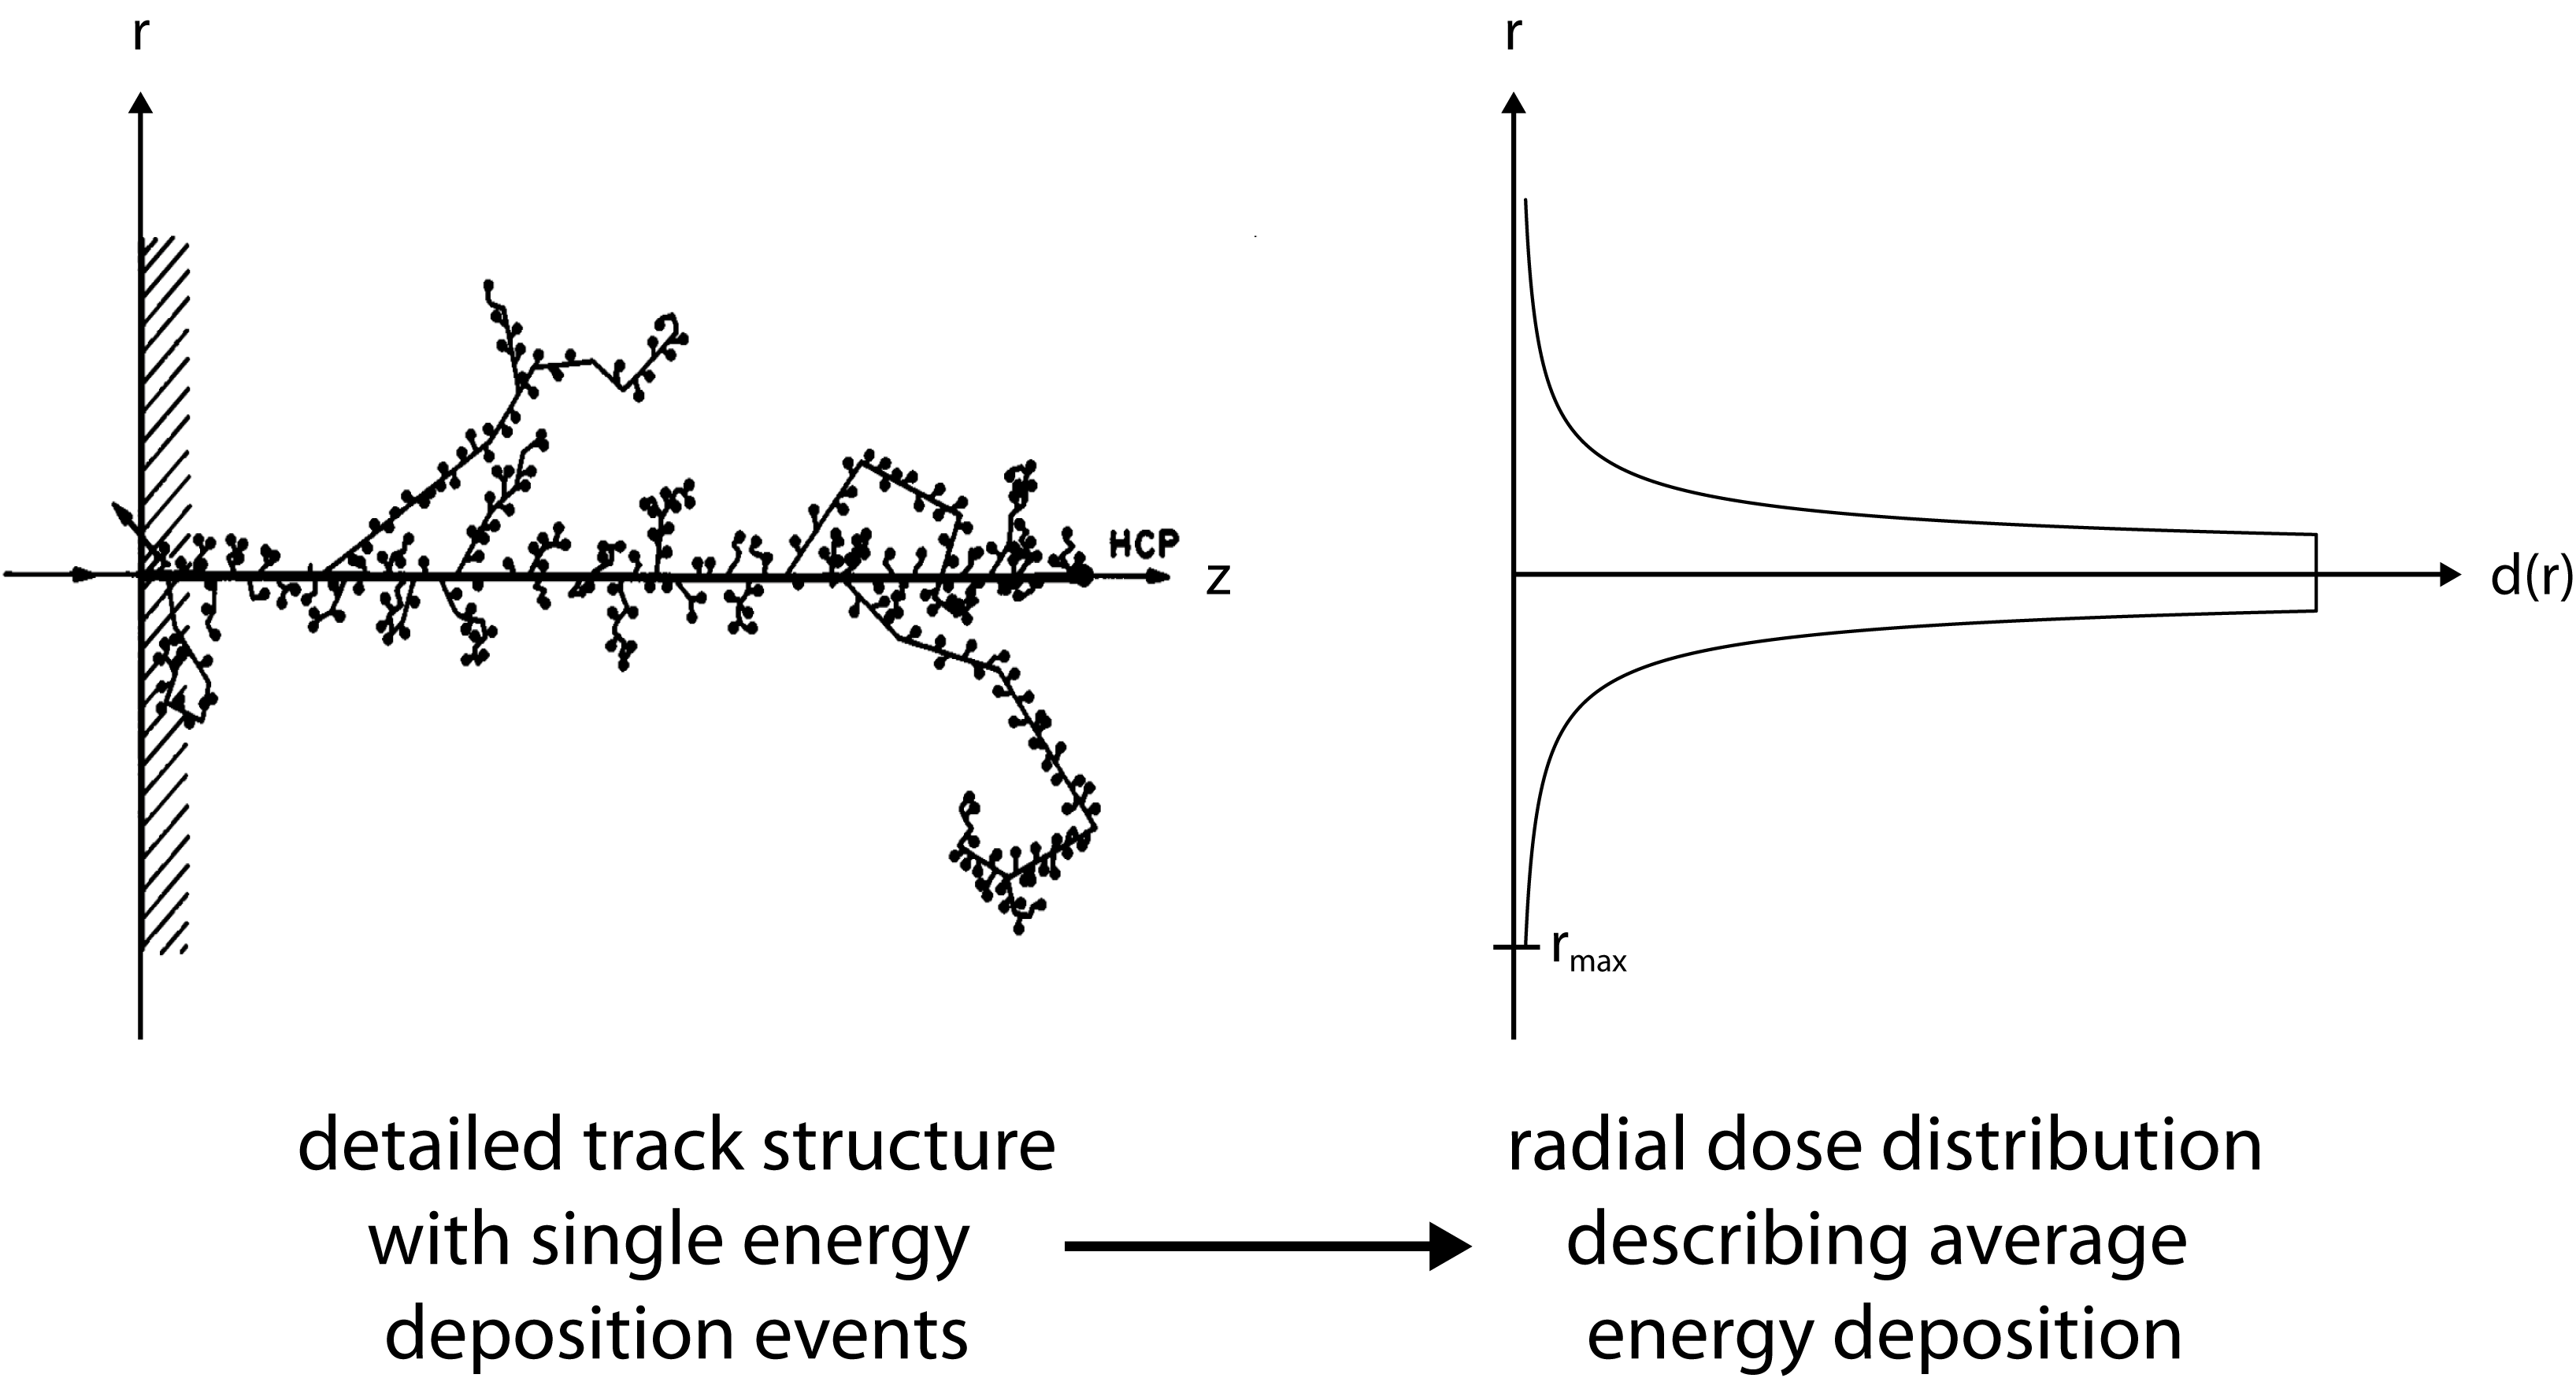
\includegraphics[width=1.0\textwidth]{pictures/TrackStructureDetailAndRDD.png}
	\caption{Amorphization of the detailed track structure.}
	\label{fig:TST}
\end{figure*}


\section{Microdosimetric models}

Theory of dual radiation action.
Olko.

\section*{Document status}
\begin{tabular}{l l}
2011.01.21&Created by S. Greilich
\end{tabular} 